
\chapter{Introdução}

%[A introdução deve, tal como o próprio nome indica, introduzir o tema do trabalho. Não deve haver pressa em falar da empresa onde foi realizado o estágio ou o curso a que se refere o trabalho. Deve fazer-se uma introdução à área, Os Sistemas Informáticos ou as Ciências da Computação são áreas bastante grandes, pelo que não se deve supor que o leitor está a par das necessidades ou das tecnologias usadas em determinada área. No entanto, não devem ser explicados conceitos básicos, que qualquer licenciado numa engenharia de sistemas informáticos ou em ciências da computação tenham obrigação de conhecer.

Acompanhar as novas tecnologias é fundamental para um negócio. É preciso investir em inovação para manter um negócio no mercado competitivo. A tecnologia, aliada a uma boa atualização, consegue proporcionar soluções eficientes às empresas.

% Algo como o resumo é valido para a introdução ???
-- por terminar -- acabaram as ideias !!

\section{ Objetivos }

% - [Numa pequena secção da introdução liste, cuidadosamente, os objetivos do trabalho. Não confundir com os requisitos do software. Apenas o que se pretendia atingir originalmente.] %

Este estágio está diretamente relacionado com o produto NkaAcademies, que se trata de uma solução web completa para a gestão de processos de formação.

%1ª opçao
%Deste modo, os principais objetivos estipulados foram a migração completa do produto NkaAcademies para as versões mais recentes do PHP e do MySQLi e posteriormente o desenvolvimento de novas funcionalidades.

%2ª opçao
Pretende-se efetuar a migração completa do produto NkaAcademies para as versões mais recentes do PHP e do MySQLi, no entanto será necessário resolver alguns problemas de compatibilidade que poderão surgir consequentemente a esta alteração e numa fase mais avançada do estágio, incorporar novas funcionalidades ao produto.

%corrigir !?!

\section{Contexto}
 %[No caso de um estágio, é nesta secção que se deverá falar da empresa em que o estágio foi realizado. Se o projeto desenvolvido faz parte de um projeto mais amplo, faz sentido que se documente os objetivos do projeto com um todo, de modo que o leitor consiga perceber onde o trabalho realizado encaixa.] %
\par Este projeto foi realizado no âmbito de estágio curricular da Licenciatura em Engenharia de Sistemas Informáticos, na empresa NKA - \textit{New Knowledge Advice} em Braga.
\par O estágio curricular teve uma duração de aproximadamente quatro meses, tendo iniciado a 22 de fevereiro e terminado a 9 junho de 2021, de segunda a quinta feira num regime maioritariamente de teletrabalho, com exceção de algumas semanas em regime presencial.
\par A NKA - \textit{New Knowledge Advice} é uma empresa tecnológica sediada em Braga, fundada em 2011 que concebe e desenvolve soluções globais vocacionadas para a otimização de cada negócio, por meio de projetos específicos, fornecendo as soluções mais adequadas às crescentes exigências dos mercados. A empresa dedica-se ainda ao desenvolvimento de software, à implementação de sistemas e à consultoria e formação\citep{nka}. 

\section{Plano de trabalhos}

No âmbito do estágio, foram identificadas as seguintes tarefas:

\begin{itemize}
    \item  Conhecer a empresa, tecnologias e projeto a desenvolver - Migração do produto NkaAcademies para as versões mais recentes do PHP e MySQLi;
    \item  Investigação sobre PHP e MySQLi - Leitura de CHANGELOG das versões anteriores. Análise de funções \textit{deprecated}.
    \item  Alteração do código para a versão 8 PHP.
    \item  Testes e correção de erros de compatibilidade
    \item  Conhecer o projeto a desenvolver - módulo auxiliar ao processo de gestão de formação.
    \item Levantamento de requisitos e funcionalidades
    \item  Desenvolvimento do módulo - Filtro de pesquisa e alteração manual e automática de documentos associados à gestão de formação.
    \item Testes e correção de erros
    \item  Preparação da aplicação - Alteração de ligações para cloud. Limpeza de código.
    \item Atualização das alterações no servidor
\end{itemize}
Para planear a execução das tarefas, foi elaborado um diagrama de Gantt de acordo com a Figura - ~\ref{fig:gantt}.

\begin{center}
        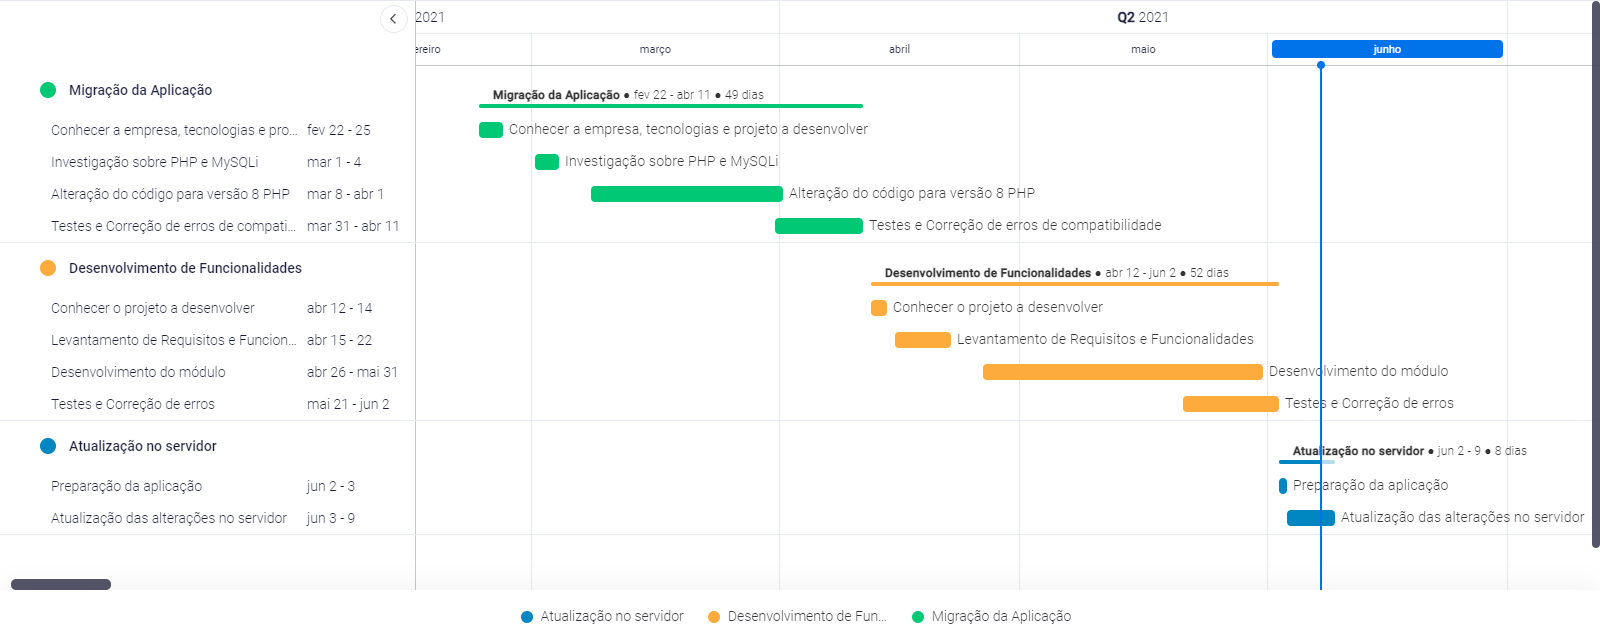
\includegraphics[width=\textwidth,height=\textheight,keepaspectratio]{images/unknown.png}
        \captionof{figure}{Diagrama de Gantt}
        \label{fig:gantt}
\end{center}


\section{Estrutura do documento}
 [A última secção da introdução deve explicar a estrutura do documento: quais são só capítulos existentes (para além do primeiro) e o que será discutido em cada um desses capítulos. A estrutura típica de um relatório de desenvolvimento de software é:

 Introdução, com um breve resumo do que se pretende atingir, e uma descrição clara dos objetivos;

\begin{enumerate}
    \item Análise ao problema, que poderá incluir uma análise ao estado da arte ou ao modelo de negócio onde se pretende intervir;
    \item Análise e modelação do sistema, em que sejam levantados sistematicamente os requisitos, descritos diagramas de caso de uso e de atividade (que descrevam/formalizem o modelo de negócio).
    \item Implementação, em que se descrevam as tecnologias escolhidas (e se justifiquem), e se refira detalhes sobre a implementação.
    \item Análise de resultados e testes, seja uma análise/avaliação aos resultados obtidos, sejam testes de usabilidade ou unitários ao trabalho desenvolvido.
    \item Conclusão.]
\end{enumerate}{}
